This thesis explores the capabilities and information of ground based lightning detection networks.
What are the limits of what lightning networks can measure?
How can these networks be expanded and what are the effects of these expansions?
Can choosing the right algorithm reveal larger structures from individual lightning strokes?

From these questions lightning, thunderstorms, and the Earth-Ionosphere system can be explored.
The electrical energy in thunderstorms is investigated in how it discharges, where the energy goes, and how does it contribute to the system as a whole.

%% Introductory text / summary / expanded abstract

\section{Background}

\subsection{Lightning and Thunderstorms}

Lightning is the discharge process of disparate charge regions in, typically, a thunderstorm.
When charge is separated in a thunderstorm, a hurricane, a volcanic ash plume, or on other planets it eventually discharges in order to neutralize the charge imbalance.
Typically this occurs through lightning flashes.

In a thunderstorm deep convection develops, lifting moist air from below the thunderstorm up through the cloud where the moisture begins to precipitate.
Figure~\ref{intro:fig:thunderstorm} shows the basic components of an active thunderstorm.
As the water droplets begin to freeze as they pass through the freezing level of the thunderstorm, at this freezing level they collide with downwelling ice particles.
At these collisions charge exchange causes the downwelling ice to gain a negative charge and the upwelling water to become positively charged.
This leads to the gross charge structure shown in Figure~\ref{intro:fig:thunderstorm}, with positive charge at the top of the thunderstorm and negative charge at the bottom.

\begin{figure}[ht!]
	\centering
	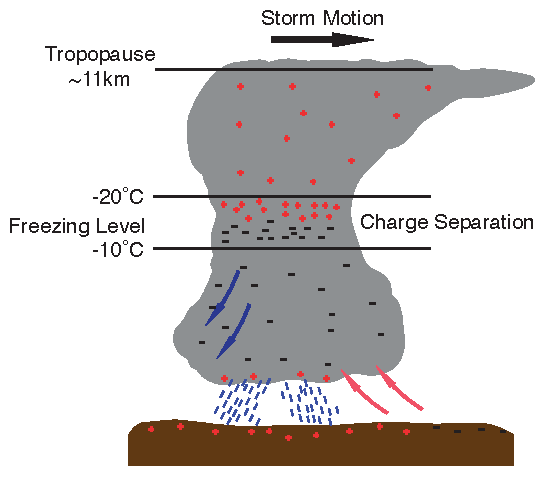
\includegraphics[scale=1]{Introduction/Figures/Thunderstorm_Structure.pdf}\\
	\caption{Overall thunderstorm structure showing the general charge distribution.}
	\label{intro:fig:thunderstorm}
\end{figure}

When enough charge is separated the stepped-leader process begins.
While an appreciable voltage builds up between the charge centers (the thunderstorm and ground for example) on the order of $MV$ it is still far less than the breakdown voltage of air.
However the air is broken down in \~100~$m$ steps that leaves an ionized plasma channel; the breakdown process is semi-fractal with steps occurring until an oppositely charge region is connected.
The process for the step-leader breakdown is shown in Figure~\ref{intro:fig:evolution}.

For the first 20~$ms$ the step leader creates the ionized channel to ground (or another charge region).
Once the channel is established the return stroke moves charge from the ground to the cloud over the course of 70~$\mu s$.
After the return stroke the top of the ionized channel can connect to other charge regions through a subsequent step-leader process producing multiple return strokes along the same channel.
The total step-leader through multiple return strokes is considered a single lightning flash.

\begin{figure}[ht!]
	\centering
	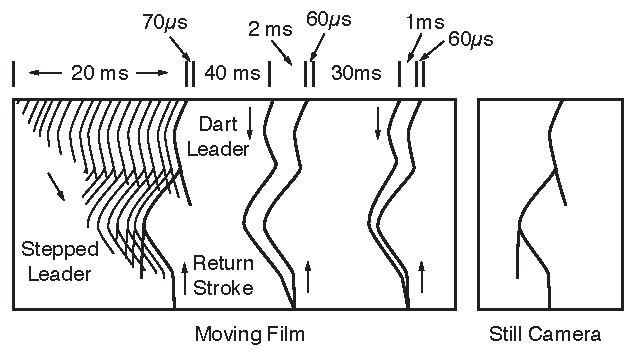
\includegraphics[scale=1]{Introduction/Figures/Lightning_Evolution.pdf}\\
	\caption{The step-leader and discharge process of cloud to ground lightning with typical times of each event.}
	\label{intro:fig:evolution}
\end{figure}

Lightning can discharge in several ways, shown in Figure~\ref{intro:fig:types}.
Predominately lightning occurs either between clouds or within the same cloud, called: cloud-to-cloud lightning, in-cloud lightning, or cloud lightning (Figure~\ref{intro:fig:types}c).
Lightning between the thunderstorm and ground is more powerful, easier to detect, and less common.
It can occur in 4 combinations of positive or negative charge in the cloud discharging to ground with the discharge beginning in the cloud or on the ground (Figure~\ref{intro:fig:types}a, \ref{intro:fig:types}b, \ref{intro:fig:types}d, and~\ref{intro:fig:types}d).
Negative cloud to ground lightning (moving negative charge from the cloud to ground, Figure~\ref{intro:fig:types}a) is the most common cloud-to-ground discharge at a ratio of 10:1.
It is estimated that are around 4 in-cloud (IC) strokes (or flashes) for every cloud-to-ground (CG) stroke.

\begin{figure}[ht!]
	\centering
	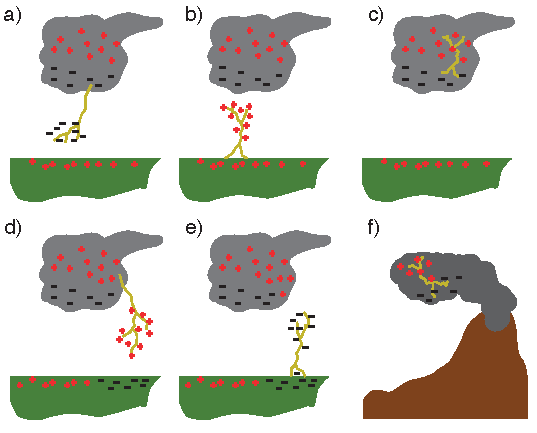
\includegraphics[scale=1]{Introduction/Figures/Lightning_Types.pdf}\\
	\caption{Different types of lightning discharges:
			a) negative cloud-to-ground,
			b) positive ground-to-cloud,
			c) in-cloud,
			d) positive cloud-to-ground,
			e) negative ground-to-cloud,
			f) volcanic ash plume.
			Note that a) and b) produce the same overall charge movement (negative charge to ground) and conversely for d) and e).}
	\label{intro:fig:types}
\end{figure}

There are other sources for large electrical discharges similar to lightning in thunderstorms.
For example there are lightning discharges in volcanic ash plumes (Figure~\ref{intro:fig:types}f), and other discharges that produce electromagnetic waves similar to lightning (terrestrial gamma ray flashes, compact intra-cloud discharges).
However these events are less common than typical lightning and will not be considered here.

\subsection{The Ionosphere}

The ionosphere is the plasma environment located between $80~km$ and 400~$km$, it is a highly conductive region with an exponentially decaying background neutral density.
It forms from the ionization of the background neutrals by ultraviolet sunlight.
During the day the ionosphere D- and E-regions extend farther down in altitude than during night when they mostly recombine and disappear.
High altitudes in the F-region remain through the night as the particle density is much lower, preventing significant recombination.
Unlike the magnetosphere it is a collisional environment.
The overall structure is shown in Figure~\ref{intro:fig:ionosphere}.

%% Add neutral density curve
%% Make better

\begin{figure}[ht!]
	\centering
	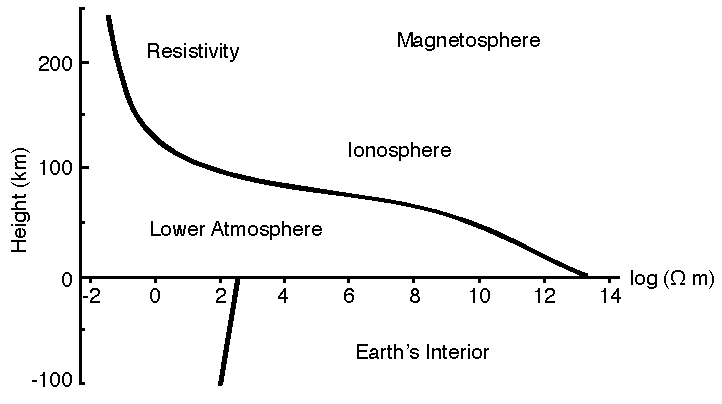
\includegraphics[scale=1]{Introduction/Figures/Atmospheric_Conductivity.pdf}\\
	\caption{Atmospheric resistivity profile shown on a log scale.}
	\label{intro:fig:ionosphere}
\end{figure}

For very low frequency waves (a 1~$Hz$ to 40~$kHz$) the conductive ionosphere and ground create the Earth-Ionosphere Wavegude (EIWG).
The EIWG allows for propagation of VLF waves from natural (lightning) and artificial (Navy VLF transmitters) to propagate great distances ($>10,000~km$).
As the VLF waves propagate in the waveguide there is loss on the order of 1~$dB/Mm$, with the loss going to heating the waveguide and the generation of plasma waves in the ionosphere (Figure~\ref{intro:fig:eiwg}).
Attenuation losses are greatest over ice, than continents, with the lowest loss over oceans.

\begin{figure}[ht!]
	\centering
	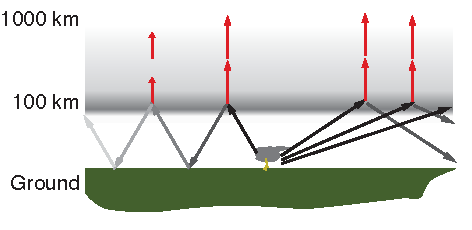
\includegraphics[scale=1]{Introduction/Figures/EIWG.pdf}\\
	\caption{Simple model of the Earth-Ionosphere Waveguide.}
	\label{intro:fig:eiwg}
\end{figure}

\subsection{Global Electric Circuit}

The global electric circuit is the current system formed by the ionosphere and ground acting as leaky spherical capacitors, as shown in Figure~\ref{intro:fig:gec}a with an equivalent circuit in Figure~\ref{intro:fig:gec}b.
Thunderstorms are the primary drivers of the circuit with the charged ionosphere discharging through fair weather.
Diurnal variation in global thunderstorm activity was original observed by \citet{Wilson1921} and \citet{Whipple1929} through a combination of thunderstorm day and electric field measurements.
Strong correlations between thunderstorm activity and fair weather return current led to the current model of the global electric circuit.
The global electric circuit changes activity changes on short time scales that are not resolved with past models or with long term averaged observations.
The global electric circuit is an important component to the solar-terrestrial system creating a link between solar activity, the ionosphere, aerosols, cloud microphysics, thunderstorms, weather, and climate \citep{Tinsley2007, Holzworth1986}.

\begin{figure}[ht!]
	\centering
	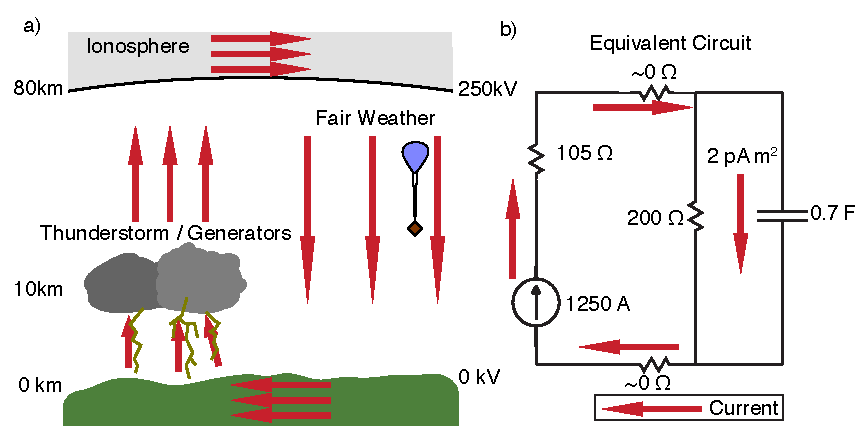
\includegraphics[scale=1]{Introduction/Figures/Global_Circuit.pdf}\\
	\caption{a) Global electric circuit model, arrow correspond to currents.
			b) Circuit equivalent model with representative values.}
	\label{intro:fig:gec}
\end{figure}

\section{Lightning Detection Systems}

There is a growing importance, both scientifically and operationally, of ground based lightning detection networks.
Lightning detection networks are being used in a larger gamut of research areas including: terrestrial gamma ray flashes \citep{Dwyer2012, Gjesteland2011, Connaughton2010}, lightning climatology \citep{Virts2013, Virts2011a, Burgesser2012}, ionospheric disturbances and probing \citep{Jacobson2010, Singh2011}, transient luminous events \citep{Soula2011}, global electric circuit  \citep{Holzworth2005}, and whistler observation \citep{Collier2010, Collier2011a, Burkholder2013}.
This is in conjunction with the extended usage of lightning networks operationally in weather prediction and tracking \citep{Fierro2012, Pan2010, Thomas2010d}, volcano monitoring \citep{Doughton2010}, and hazard estimation \citep{Altaratz2010}.
With growing usage it is necessary to understand the capabilities and efficiencies of the various available lightning networks.

Ground based total lightning networks distinguish themselves from other ground based networks and satellites by detecting and identifying in-cloud (IC) discharges as well as cloud to ground (CG) strokes.
Lightning type is critical in understanding thunderstorm dynamics \citep{Williams1989}, with real time monitoring of sudden increases of IC activity able to predict severe weather events \citep{Rudlosky2013, Darden2010, Metzger2013, Schultz2009, Schultz2011}.
The higher frequencies of total lightning networks are also useful for researching narrow bipolar events \citep{Suszcynsky2003} and large scale lightning behavior \citep{Hutchins2013}.
Lightning mapping arrays are able to locally detect, locate, and distinguish IC activity, however total lightning networks have the advantage of much larger spatial coverage.

\subsection{World Wide Lightning Location Network}

%% Add in global stroke distribution figure

%% Update with more recent papers
The World Wide Lightning Location Network (WWLLN, see http://wwlln.net) determines the location for nearly all lightning producing storms around the globe in real time (c.f. \citet{Jacobson2006c}).
WWLLN has been generating global lightning locations starting in 2004 \citep{Rodger2006, Rodger2009}.
Since then the network has grown from 18 stations to over 70 as of September 2013.
Knowledge of individual stroke locations, with high temporal accuracy, and within a fraction of a wavelength is beneficial for both scientific and technical uses.
WWLLN lightning location data have recently been used for advances in space science \citep{Lay2007, Kumar2009, Collier2009, Holzworth2011, Jacobson2011}, meteorology \citep{Price2009,Thomas2010d}, detailed lightning physics \citep{Connaughton2010}, and volcanic eruption monitoring \citep{Doughton2010}.

The network uses a time of group arrival (TOGA) technique, originally developed by \citet{Dowden2002d}, to locate strokes by analyzing the sferic waveforms at each station using the Stroke\_B algorithm as discussed by \citet{Rodger2006,Rodger2009}.
WWLLN locates strokes by analyzing the TOGA of the sferic wave packet in the 6 -- 18~kHz band \citep{Dowden2000}.
The TOGA of the VLF wave packet, is used rather than ``trigger time'' to produce more uniform arrival times across the network.
A recent upgrade to the network allows for the measurement of the radiated VLF energy of located strokes within the 8 -- 18~kHz VLF band.
The stroke energy is calculated from the time-integrated root mean square (RMS) electric field of the VLF sferic at each WWLLN station, using the Long Wave Propagation Capability code (LWPC) \citep{Ferguson1998} to estimate the sferic attenuation and calculate the source radiated energy \citep{Hutchins2012}.

As stations are added the accuracy and detection efficiency of the network improves.
As of 2010 the network locates most strokes to within 10 kilometers and $<$10~$\mu$s with an estimated detection efficiency of about 11\% for all strokes and $>$30\% for more powerful strokes \citep{Abarca2010,Rodger2009}.
The network improves in accuracy and detection efficiency with increased stations; for example an increase in the number of WWLLN stations from 11 in 2003 to 30 in 2007 led to a $\sim$165\% increase in the number of lightning strokes located \citep{Rodger2009}.
However the WWLLN network does not observe lightning with the same detection efficiency everywhere.
This is due to variable WWLLN station coverage and the strong affect on VLF radio propagation from orography and ionospheric conditions along the great circle path of a wave.

\subsection{Earth Networks Total Lightning Network}

%% Add ENTLN stroke density figure

The Earth Networks Total Lightning Network (ENTLN) is a ground based network that began in 2009 as the Weatherbug Total Lightning Network (WTLN).
It has two operational regimes: short range using broadband sferic waveforms (5~kHz -- 12~MHz) and long range with only VLF waveforms (1~Hz -- 256~kHz) \citep{Heckman2010}.
Correlations of the stroke waveform and amplitude from multiple stations determines the time, location, altitude, peak current, polarity, and type of the located stroke \citep{Liu2011a}.
The network utilizes a time of arrival method to determine the location of each stroke, where a minimum of 8 stations is required to produce a valid solution.
To compress the broadband waveforms each station removes the necessary amount of low-amplitude signal to reach the requisite packet size.
In the continental United States (CONUS) the network has approximately 530 operational stations in September 2013.
A comparison to the Oklahoma Lightning Mapping Array (OKLMA) in 2010 demonstrated the ability to discriminate between CG and IC strokes \citep{Beasley2010}.

\subsection{TRMM/LIS}

%% Add LIS global flash count figure.

The Lightning Imaging Sensor (LIS, 1997-present) is a satellite-based lightning detector flown onboard the Tropical Rainfall Measurement Mission (TRMM) satellite orbiting at a 35$^\circ$ inclination and 402~km altitude \citep{Christian1999}.
In low earth orbit it observes the total lightning activity from individual thunderstorms for 90 sec in each $0.5^\circ \times 0.5^\circ$ viewtime granule.
LIS is useful as it is a lightning detection system with no overlapping detections methods with ground based networks, and the sensor performance has not changed over time.
The LIS data are available at several processed levels, throughout this work the flash level data is used.

\section{Long Wave Propagation Capability Code}

The Long Wave Propagation Capability code (LWPC) is used to model the VLF attenuation between WWLLN located lightning and the network stations.
The LWPC code was developed by the Space and Naval Warfare Systems Center by \citet{Ferguson1998} and has most recently been validated by \citet{McRae2000d, Thomson2011}.
In this research we made use of an adapted LWPC version 2.1.

LWPC can be used to model the attenuation along a mixed day/night ionospheric path, however due to computational limitations a lookup table is used instead.
The lookup tables model the received electric field at a given station for a 100~kW transmitter in each grid cell.
A $1^{\circ}$ by $1^{\circ}$ grid is used for either an all day ($\beta=0.3$ km$^{-1}$ and $h'=74$ km) or an all night ($\beta(f)=0.3-0.8$ km$^{-1}$ and $h'=87$ km) ionospheric model, where $\beta$ and $h'$ are the slope of the conductivity ($\beta$ is frequency dependent at night) and the reference height in the ionospheric model.
The ionospheric models are the default models of LWPC code and fully described in \citet{Ferguson1998}. 

For each grid cell the electric field is averaged over the 8 -- 18 kHz band, which captures the frequencies of the peak radiated power from lightning \citep{Volland1995}.
An example of the day ionosphere lookup table for the Dunedin station is shown in Figure~\ref{intro:fig:lookup} (reproduced from Chapter~\ref{thesis:chapter:efficiency}).
The discontinuity of electric field over Greenland and in the South Atlantic is caused by the high attenuation rate of VLF propagating over ice.
Using the lookup tables assumes that the attenuation rates do not vary greatly within a given grid cell and that the frequency spectra of a sferic is relatively flat within the band considered.

\begin{figure}[ht!]
	\centering
	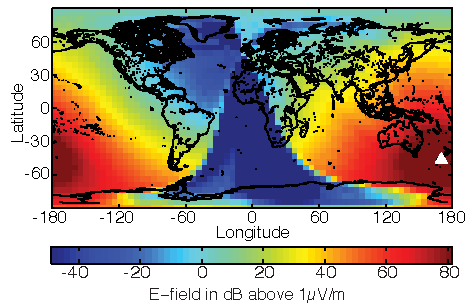
\includegraphics[scale=1]{energy/Figures/PPS_Lookup.pdf}\\
	\caption{LWPC generated lookup table for Dunedin station (white triangle) using an all day ionospheric model ($	\beta=0.3$ km$^{-1}$ and $h'=74$ km) averaged over 8-18 kHz. Each $1^{\circ}$ by $1^{\circ}$ bin shows the electric field seen at Dunedin if a 100kW transmitter is centered on that bin.}
	\label{intro:fig:lookup}
\end{figure}

\section{Outline}

In Chapter~\ref{thesis:chapter:energy} the process for calculating the far-field radiated VLF energy of lightning with WWLLN is described.
The work is adapted from the \citet{Hutchins2012} paper.
Chapter~\ref{thesis:chapter:efficiency} discusses the relative detection efficiency model of WWLLN.
The work is from the \citet{Hutchins2012a} paper.
The network improvements of Chapters~\ref{thesis:chapter:energy} and~\ref{thesis:chapter:efficiency} enables the work in Chapters~\ref{thesis:chapter:landsea} and~\ref{thesis:chapter:landsea}.

Chapter~\ref{thesis:chapter:landsea} examines the contrast between oceanic and continental lightning using the WWLLN stroke energy measurements with a linear regression method developed in the chapter.
This research is adapted from the \citet{Hutchins2013}.
Chapter~\ref{thesis:chapter:prop} combines the WWLLN energy measurements with the LWPC code to estimate the VLF attenuation rates over ocean in the day and night ionospheric regimes.
This research is adapted from the \citet{Hutchins2013a}.
Chapter~\ref{thesis:chapter:gec} applies a clustering algorithm to the WWLLN stroke locations, producing thunderstorm clusters, to create a prediction of the global electric circuit activity.
%% Update status as needed
This research is currently submitted and under review.

Appendix~\ref{thesis:appendix:code} describes the different types of WWLLN data files available, their location, and the common code used in this thesis (code for individual chapters can be made available upon request).
Notably the code for the energy calculations (Chapter~\ref{thesis:chapter:energy}), relative detection efficiency model (Chapter~\ref{thesis:chapter:efficiency}), and thunderstorm clustering (Chapter~\ref{thesis:chapter:gec}) are available online.
Appendix~\ref{thesis:appendix:energy} describes the WWLLN stroke energy code and operations, enabling both reproduction of the results and steps to setup new energy processing computers.

Appendix~\ref{thesis:appendix:su} and~\ref{thesis:appendix:gumstix} describe the development, construction, and operation of the WWLLN Service Unit v4 computers.
Schematics, EAGLE files, parts list, software, and operations are all described with the code available as described in Appendix~\ref{thesis:appendix:code}.
